\section{Oscilador de Wien}
\subsection{Introducción}
Las señales senoidales son de vital importancia en el ámbito de la electrónica, tanto en usos de intercambio de información como transferencia de energía, entre otros, y 
es justamente por eso que la generación de las mismas es de real importancia.
Una forma de generar señales senoidales mediante componentes analógicos electrónicos es mediante osciladores, y uno de los ejemplos de estos circuitos es el oscilador de 
Wien, cuya forma más elemental se muestra en la Figura \ref{fig:basic_wien_osc}.
\begin{figure}[H]
    \centering
    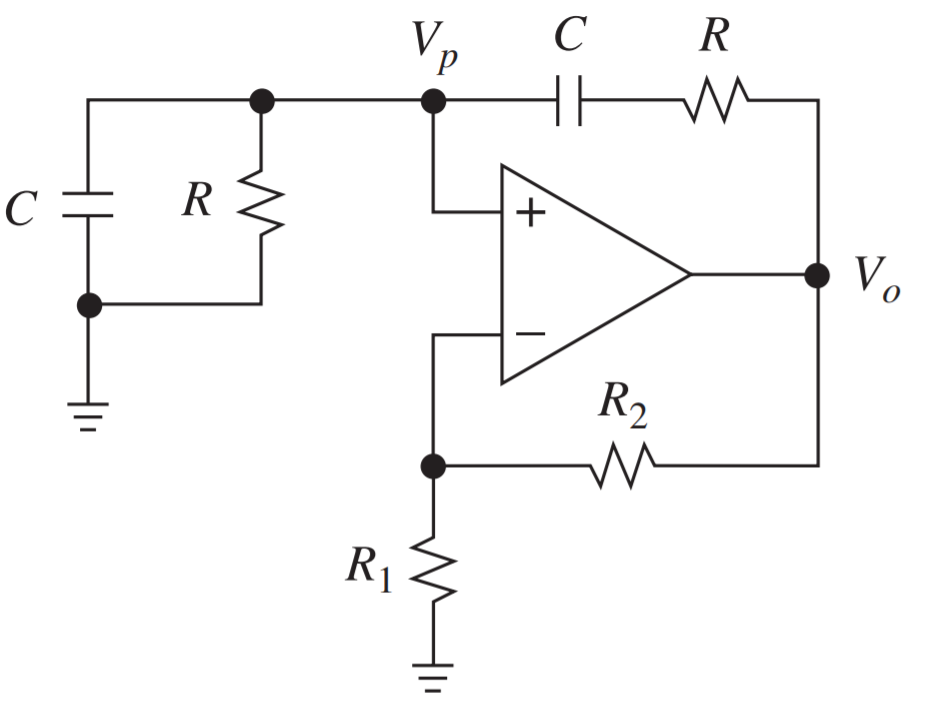
\includegraphics[width=0.5\textwidth]{../EJ1/Recursos/basic_wien_osc.png}
    \caption{Oscilador de Wien en su forma más sencilla.}
    \label{fig:basic_wien_osc_ex1}
\end{figure}
El objetivo de esta sección del artículo es, basándose en derivaciones del circuito anterior, diseñar un oscilador que genere una señal senoidal con su frecuencia de 
oscilación en $77.5KHz$ como único parámetro de diseño.



\subsection{Marco teórico}
\subsubsection{Frecuencia de oscilación}
Retomando el circuito planteado en la sección anterior, el mismo puede ser analizado para encontrar las relaciones que determinan el los parámetros fundamentales de la 
señal generada por el oscilador.
El mismo puede ser pensado como un amplificador realimentado tanto positiva como negativamente, donde el lazo negativo es el de un amplificador no inversor de ganancia:
\begin{align} 
    & A = 1 + \frac{R_2}{R_1}
    \label{eq:neg_loop_gain_ex1}
\end{align}

La tensión de entrada a este no inversor puede ser puesta en función de los parámetros del lazo negativo mediante la ecuación \ref{eq:v_p_by_v_o_ex1}.
\begin{align*}
    & V_p = V_o \frac{R // \frac{1}{j \cdot 2\pi \cdot f \cdot C}}{\left( R // \frac{1}{j \cdot 2\pi \cdot f \cdot C} \right) + \left( R + \frac{1}{j \cdot 2\pi \cdot f \cdot C}\right)}
\end{align*}
Manipulando algebraicamente esta expresión se obtiene la ganancia debida al lazo positivo:
\begin{align}
    & B(jf) = \frac{1}{3 + j \cdot \left(\frac{f}{f_0} - \frac{f_0}{f}\right)}
    \label{eq:pos_loop_gain_ex1}
\end{align}
Donde:
\begin{align}
    & f_0 = \frac{1}{j \cdot 2\pi \cdot R \cdot C}
    \label{eq:osc_freq_ex1}
\end{align}

La ganancia total del oscilador viene dada por la multiplicación de las ganancias de los lazos, consecuentemente, de las ecuaciones \ref{eq:neg_loop_gain_ex1} y \ref{eq:pos_loop_gain_ex1}
se obtiene:
\begin{align}
    & T(jf) = \frac{1 + \frac{R_2}{R_1}}{3 + j \cdot \left(\frac{f}{f_0} - \frac{f_0}{f}\right)}
    \label{eq:total_gain_ex1}
\end{align}

De la observación de esta transferencia puede deducirse que se trata de un pasa banda con ganancia máxima en $f = f_0$ y ganancia:
\begin{align}
    & T_{max} = \frac{1 + \frac{R_2}{R_1}}{3}
    \label{eq:max_gain_ex1}
\end{align}


\subsubsection{Criterio de Barkhausen}
El criterio de Barkhausen dicta las condiciones que deben cumplirse en oscilador como el de Wien para que se cumpla la condición de oscilación y determina la frecuencia a 
la que se dará el mismo.
El criterio consiste en hallar el punto para el cual se cumple que la ganancia es 1 y el desfasaje es nulo, y, para el circuito en cuestión, observamos que la segunda de 
las condiciones puede ser cumplida evaluando en $f_0$, mientras que la primera puede cumplirse para esa misma frecuencia si $\frac{R_2}{R_1} = 2$


\subsubsection{Desviaciones del circuito básico}



\subsection{Diseño y función de los componentes}
\subsubsection{Lazo de realimentación positiva}


\subsubsection{Lazo de realimentación negativa}


\subsubsection{Diodo rectificador y diodo Zener}


\subsubsection{Transistor JFET}


\subsubsection{Polarización del JFET ($C_3$ y $R_x$)}


\subsubsection{Selección del operacional a utilizar}



\subsection{Caracterización del sistema}
\subsubsection{Singularidades}


\subsubsection{Sensibilidades}



\subsection{Resultados}
\subsubsection{Frecuencia de oscilación}


\subsubsection{Tensión de salida}


\subsubsection{Establecimiento de la señal}


\subsubsection{Distorsión armónica}
